
\documentclass{webofc}

% Package imports go here.
\usepackage[varg]{txfonts}
\usepackage{amsmath,amsfonts,amssymb}
\usepackage{graphicx}
\usepackage{orcidlink}
\usepackage{listings}
\usepackage{xcolor}
\usepackage{longtable}

% Local commands go here.
\newcommand{\aj}{AJ}
\newcommand{\apj}{ApJ}
\newcommand{\apjl}{Astrophys. J. Lett.}
\newcommand{\apjs}{ApJS}
\newcommand{\procspie}{Proc.\ SPIE}
\newcommand{\pasj}{PASJ}
% lsstdoc documentation: https://lsst-texmf.lsst.io/lsstdoc.html
\input{meta}

% Package imports go here.

% Local commands go here.
\graphicspath{{./figures/}} 

\newcommand{\docRef}{DMTN-356}
\newcommand{\docUpstreamLocation}{\url{https://github.com/lsst-dm/dmtn-356}}


\begin{document}
\title{From Petabytes to Discovery: The Computing Ecosystem Powering Rubin Observatory's LSST}

% This can write metadata into the PDF.
% Update keywords and author information as necessary.
\hypersetup{
    hidelinks,
    pdftitle={From Petabytes to Discovery: The Computing Ecosystem Powering Rubin Observatory's LSST},
    pdfauthor={guylp},
    pdfkeywords={}
}

\input{authors}

\abstract{The Vera C. Rubin Observatory began the Legacy Survey of Space and Time (LSST), a ten-year optical survey of the southern sky, on 30 June 2026. This paper presents early Rubin images and discoveries, focusing on the data management system that makes science at this scale possible. Building on  LHC-scale distributed computing experience, Rubin deploys HEP tools, including Rucio and FTS for data movement, CernVM-FS for software distribution and HTCondor for workflow management at its three data facilities: SLAC, an ATLAS Tier-2 site, and the France and UK facilities, both long-standing LHC Tier-1 centres.  We describe the end-to-end Rubin computing ecosystem, present early science results, and discuss lessons from the astronomy--HEP collaboration and open challenges for high-volume, high-rate astronomical surveys.

}

\maketitle

% ============================================================
\section{Introduction}
\label{sec:intro}
% ============================================================

On 30~June~2026, the NSF--DOE Vera C.\ Rubin Observatory began the Legacy Survey of Space and Time (LSST), a ten-year, wide-field optical survey of the southern sky that will produce the deepest and most complete time-domain map of the Universe to date. 
The observatory was named by Act of the US Congress in December 2019 for Vera C.\ Rubin (1928--2016), whose measurements of galaxy rotation curves provided compelling evidence for dark matter, and who was a tireless advocate for women in science. It is the first US national observatory named for a woman.

Rubin works very differently from a traditional observatory. 
At a pointed facility such as Gemini or Keck, a principal investigator (PI) proposes for time to answer a specific question; data volumes are modest, and the PI downloads the resulting dataset to analyse locally. 
LSST has no PI-driven programs. 
The sky is imaged according to a survey strategy developed with the global scientific community~\cite{PSTN-055}, and observations are selected in
real time by the Feature Based Scheduler (FBS), an automated decision-making system built on a Markov decision process framework~\cite{2026SPIE14151E..0XJ}.
Roughly every 30~s, the FBS ingests telemetry on the observatory, sky and weather, and selects the next pointing from about 1500 candidates by maximising a weighted reward that balances expected image depth, slew time and progress towards the desired footprint coverage. 
Each night, Rubin produces $\sim$10~TB of raw images and up to 10~million transient alerts, issued within 120~s of shutter close.
Separately, all images acquired to date are reprocessed approximately annually into a single dataset, released as a Data Release, that enables multiple independent science programs across a global community of $\sim$7500 scientists.

To the high-energy physics (HEP) community, this picture is familiar.
 A large LHC experiment is trigger-driven rather than proposal-driven, relies on fully automated reconstruction, and produces a common dataset shared by the whole collaboration: the same data underpin Higgs measurements, B-physics, top-quark properties and searches for physics beyond the Standard Model. 
Likewise, science ranging from near-Earth asteroids and interstellar visitors in the Solar System, through variable stars, supernovae and active galactic nuclei, to galaxy evolution, dark energy and dark matter is served by the same LSST images and catalogs~\cite{2019ApJ...873..111I}.
Processing runs automatically across three international data facilities, and scientists access the results through the Rubin Science Platform (RSP), bringing their analysis to the data rather than downloading it.
In these respects, Rubin has more in common with an LHC experiment than with pointed astronomy.

Recognising this, Rubin looked to established HEP tools, including Rucio~\cite{2019CSBS....3...11B}, PanDA~\cite{2024EPJWC.29504026K}, HTCondor and CernVM-FS~\cite{2011JPhCS.331d2003B}, rather than building astronomy-specific infrastructure from scratch.
The choice was also a practical one: all three Rubin data facilities are Worldwide LHC Computing Grid (WLCG) sites.
SLAC National Accelerator Laboratory (USDF), the lead Rubin data facility and archive centre is an ATLAS Tier-2 site, the French facility (FrDF) (CC-IN2P3, an LHC Tier-1 centre) and the UK facility (UKDF) (RAL, an LHC Tier-1 centre, together with the GridPP Tier-2 site at Lancaster) are long-standing WLCG centres, each with operational experience of these tools and the networks needed for petabyte-scale data movement.
During commissioning and early operations, these tools are being evaluated for multi-site Data Release Processing (DRP) for the full LSST, starting with Data Release 1 (DR1), expected in 2028.
Rubin has drawn on more than a decade of HEP operational experience at petabyte scale, and in turn is extending these tools to new storage paradigms and computing environments.

This paper describes the end-to-end Rubin computing ecosystem as it stands at the start of LSST operations, highlights early scientific results, and discusses lessons learned and open challenges for modern high-volume, high-rate astronomical surveys.

% ============================================================
\section{Rubin Observatory}
\label{sec:rubin_obs}
% ============================================================

Rubin Observatory is a dedicated survey facility, jointly funded by the US National Science Foundation and the US Department of Energy Office of Science, on Cerro~Pach\'{o}n in northern Chile.
The 2647~m site offers dark, dry and stable skies, more than 300 clear nights per year, and access to the Galactic centre and the Magellanic Clouds.
The scientific vision behind Rubin Observatory and the LSST was pioneered by J.\ Anthony Tyson (UC Davis), who proposed the Dark Matter Telescope~\cite{2001ASPC..237..417T}, a wide-area survey to map dark matter and explore the time-domain Universe.
Such a survey requires a large aperture, a very wide field of view, and the agility to move rapidly between fields.
Correcting spherical aberration, coma, and astigmatism over a wide field requires three mirrors, but classical three-mirror designs spread the mirrors far apart, giving a long, slow structure.
Roger Angel (University of Arizona) recognised that the primary (M1) and tertiary (M3) mirrors could be cast and polished from a single borosilicate blank.
This keeps the 8.4~m, $\sim$300-tonne Simonyi Survey Telescope~\cite{2024SPIE13094E..09S} short and stiff, so that it can slew $3.5^\circ$ and settle in about 4~s before the next 30~s exposure, revisiting the visible sky every 3--4 nights.
%

The 3.2-gigapixel LSST Camera (LSSTCam)~\cite{2024SPIE13096E..1OL,2024SPIE13096E..1SR}, the largest digital camera ever built, covers 9.6~deg$^2$ per exposure, about 45 times the area of the full Moon, through six broad-band filters ($ugrizy$, 320--1050~nm).

Together, the telescope and camera give Rubin an \'etendue\footnote{The product of effective collecting area and field of view.} of 319~m$^2$\,deg$^2$~\cite{2019ApJ...873..111I}, the largest of any optical survey facility built to date.
\'Etendue is the survey-astronomy equivalent of instantaneous luminosity in collider physics: it sets the rate at which a facility accumulates data, and hence how quickly rare events become statistically accessible.
The compact M1M3 design is central to this survey power: keeping the 300-tonne structure short and stiff delivers both the large collecting area and the 4~s slew-and-settle cycle that together sustain the cadence.

The Data Management System (\S\ref{sec:ecosystem}) turns the resulting data stream into a single science-ready dataset that serves all of the science described in \S\ref{sec:survey}, much as one ATLAS or CMS dataset serves an experiment's entire physics program.
Rubin also runs a dedicated Education and Public Outreach program~\cite{2014SPIE9150E..14B}, whose Rubin Sky Viewer\footnote{\url{https://skyviewer.rubinobservatory.org}} gives anyone full-resolution, interactive access to Rubin images in a web browser.

% ============================================================
\section{The Legacy Survey of Space and Time}
\label{sec:survey}
% ============================================================
%
LSST is built around four science pillars, chosen specifically because they place complementary demands on depth, area, cadence and alert latency: probing dark energy and dark matter, taking an inventory of the Solar System, exploring the transient optical sky, and mapping the Milky Way~\cite{2019ApJ...873..111I}.
Over ten years, LSST is expected to detect $\sim$20~billion galaxies, $\sim$17~billion stars and $\sim$6~million Solar System objects.
The instrument and cadence are optimised for all four pillars together rather than for any one programme, and the survey and DMS deliver a single dataset that serves them all, just as one ATLAS or CMS dataset serves studies of the Higgs boson, QCD, dark matter, flavour physics and electroweak precision.

The baseline survey~\cite{PSTN-055}, shown in figure~\ref{fig:survey-map}, devotes $\sim$80--90\% of the time to the Wide-Fast-Deep (WFD) survey, covering $\sim$18\,000~deg$^2$ with $\sim$800 visits per pointing to a coadded depth of $r\sim27.5$.
Five Deep Drilling Fields take $\sim$7\% and reach $r\sim28$; mini- and micro-surveys ($\sim$1--10\%) cover the northern ecliptic, the Galactic plane and other specialised regions; and $\sim$3\% is reserved for Target of Opportunity follow-up~\cite{RTN-098} of gravitational-wave and high-energy neutrino events.
Localisation regions of tens to hundreds of square degrees must be searched within hours to catch a fading kilonova, and Rubin's combination of wide field and depth makes it uniquely suited to finding these faint, rapidly evolving optical counterparts.

LSST data is used by $\sim$7500 scientists in $\sim$30 countries, organised into eight Science Collaborations\footnote{\url{https://rubinobservatory.org/for-scientists/science-collaborations}} supported by the LSST Discovery Alliance\footnote{\url{https://lsstdiscoveryalliance.org}}.

\begin{figure}[htb]
\centering
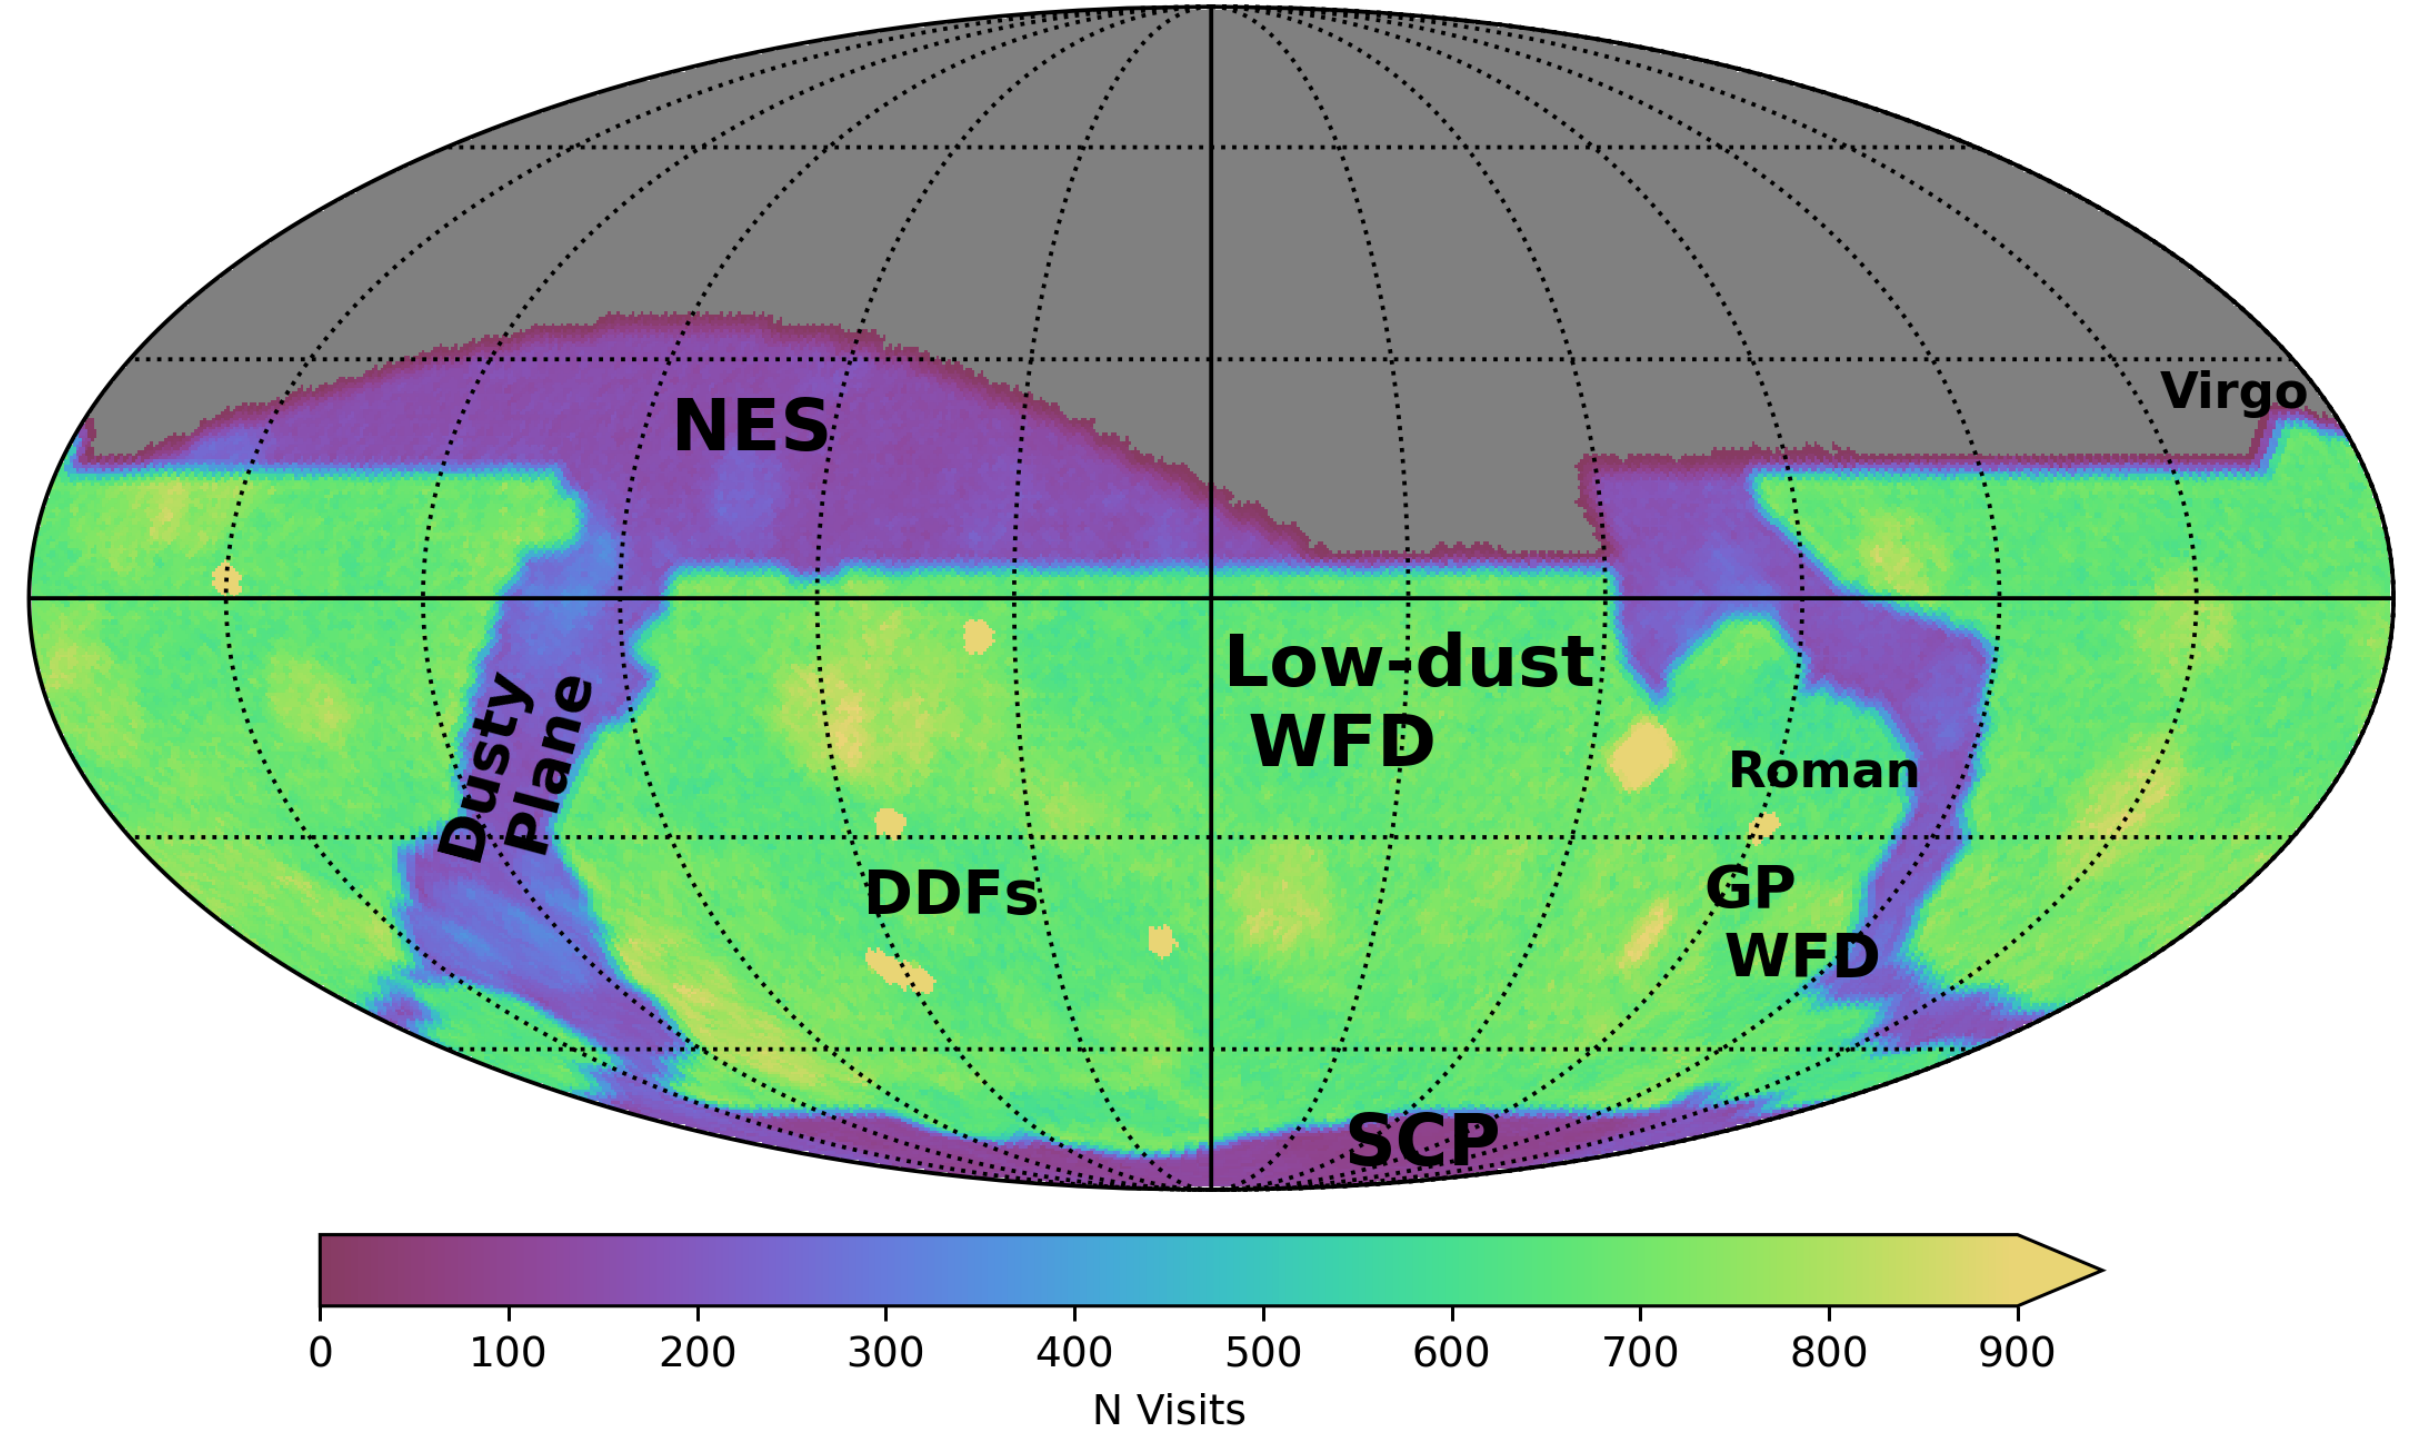
\includegraphics[width=0.85\columnwidth,clip]{baseline_v5.3.0_10yrs_nvisits_compact}
\caption{The LSST baseline survey footprint on the sky.
The wide-fast-deep main survey covers $\sim$18\,000~sq~deg of the southern sky; the five Deep Drilling Fields and supplementary mini-surveys are overlaid.}
\label{fig:survey-map}
\end{figure}

% ============================================================
\section{Early Science from LSSTCam Commissioning}
\label{sec:science}
% ============================================================

LSSTCam saw first photons on 15~April~2025, and on 23~June~2025 Rubin released its first public images in the ``First Look'' campaign, designed to showcase Rubin's unique combination of wide field, depth and speed.
Both First Look images were processed with the LSST Science Pipelines (\S\ref{sec:pipelines}), making them a commissioning exercise as well as a scientific demonstration.
The first combines 678 exposures of the Trifid and Lagoon Nebulae, taken over just 7.2~hours, into a $\sim$5-gigapixel mosaic (Figure~\ref{fig:trifid}), showing how quickly Rubin builds depth: faint gas and dust in a crowded Galactic field, revealed in a single night.
The second, the ``Cosmic Treasure Chest'', combines 1185 images of $\sim$25~deg$^2$ of the southern Virgo Cluster taken over seven nights (Figure~\ref{fig:treasure}), showing the combination of area and depth: $\sim$10~million galaxies, from bright cluster members to faint, distant background galaxies, in a region only a few times the camera's field of view.
%
\begin{figure}[htb]
\centering
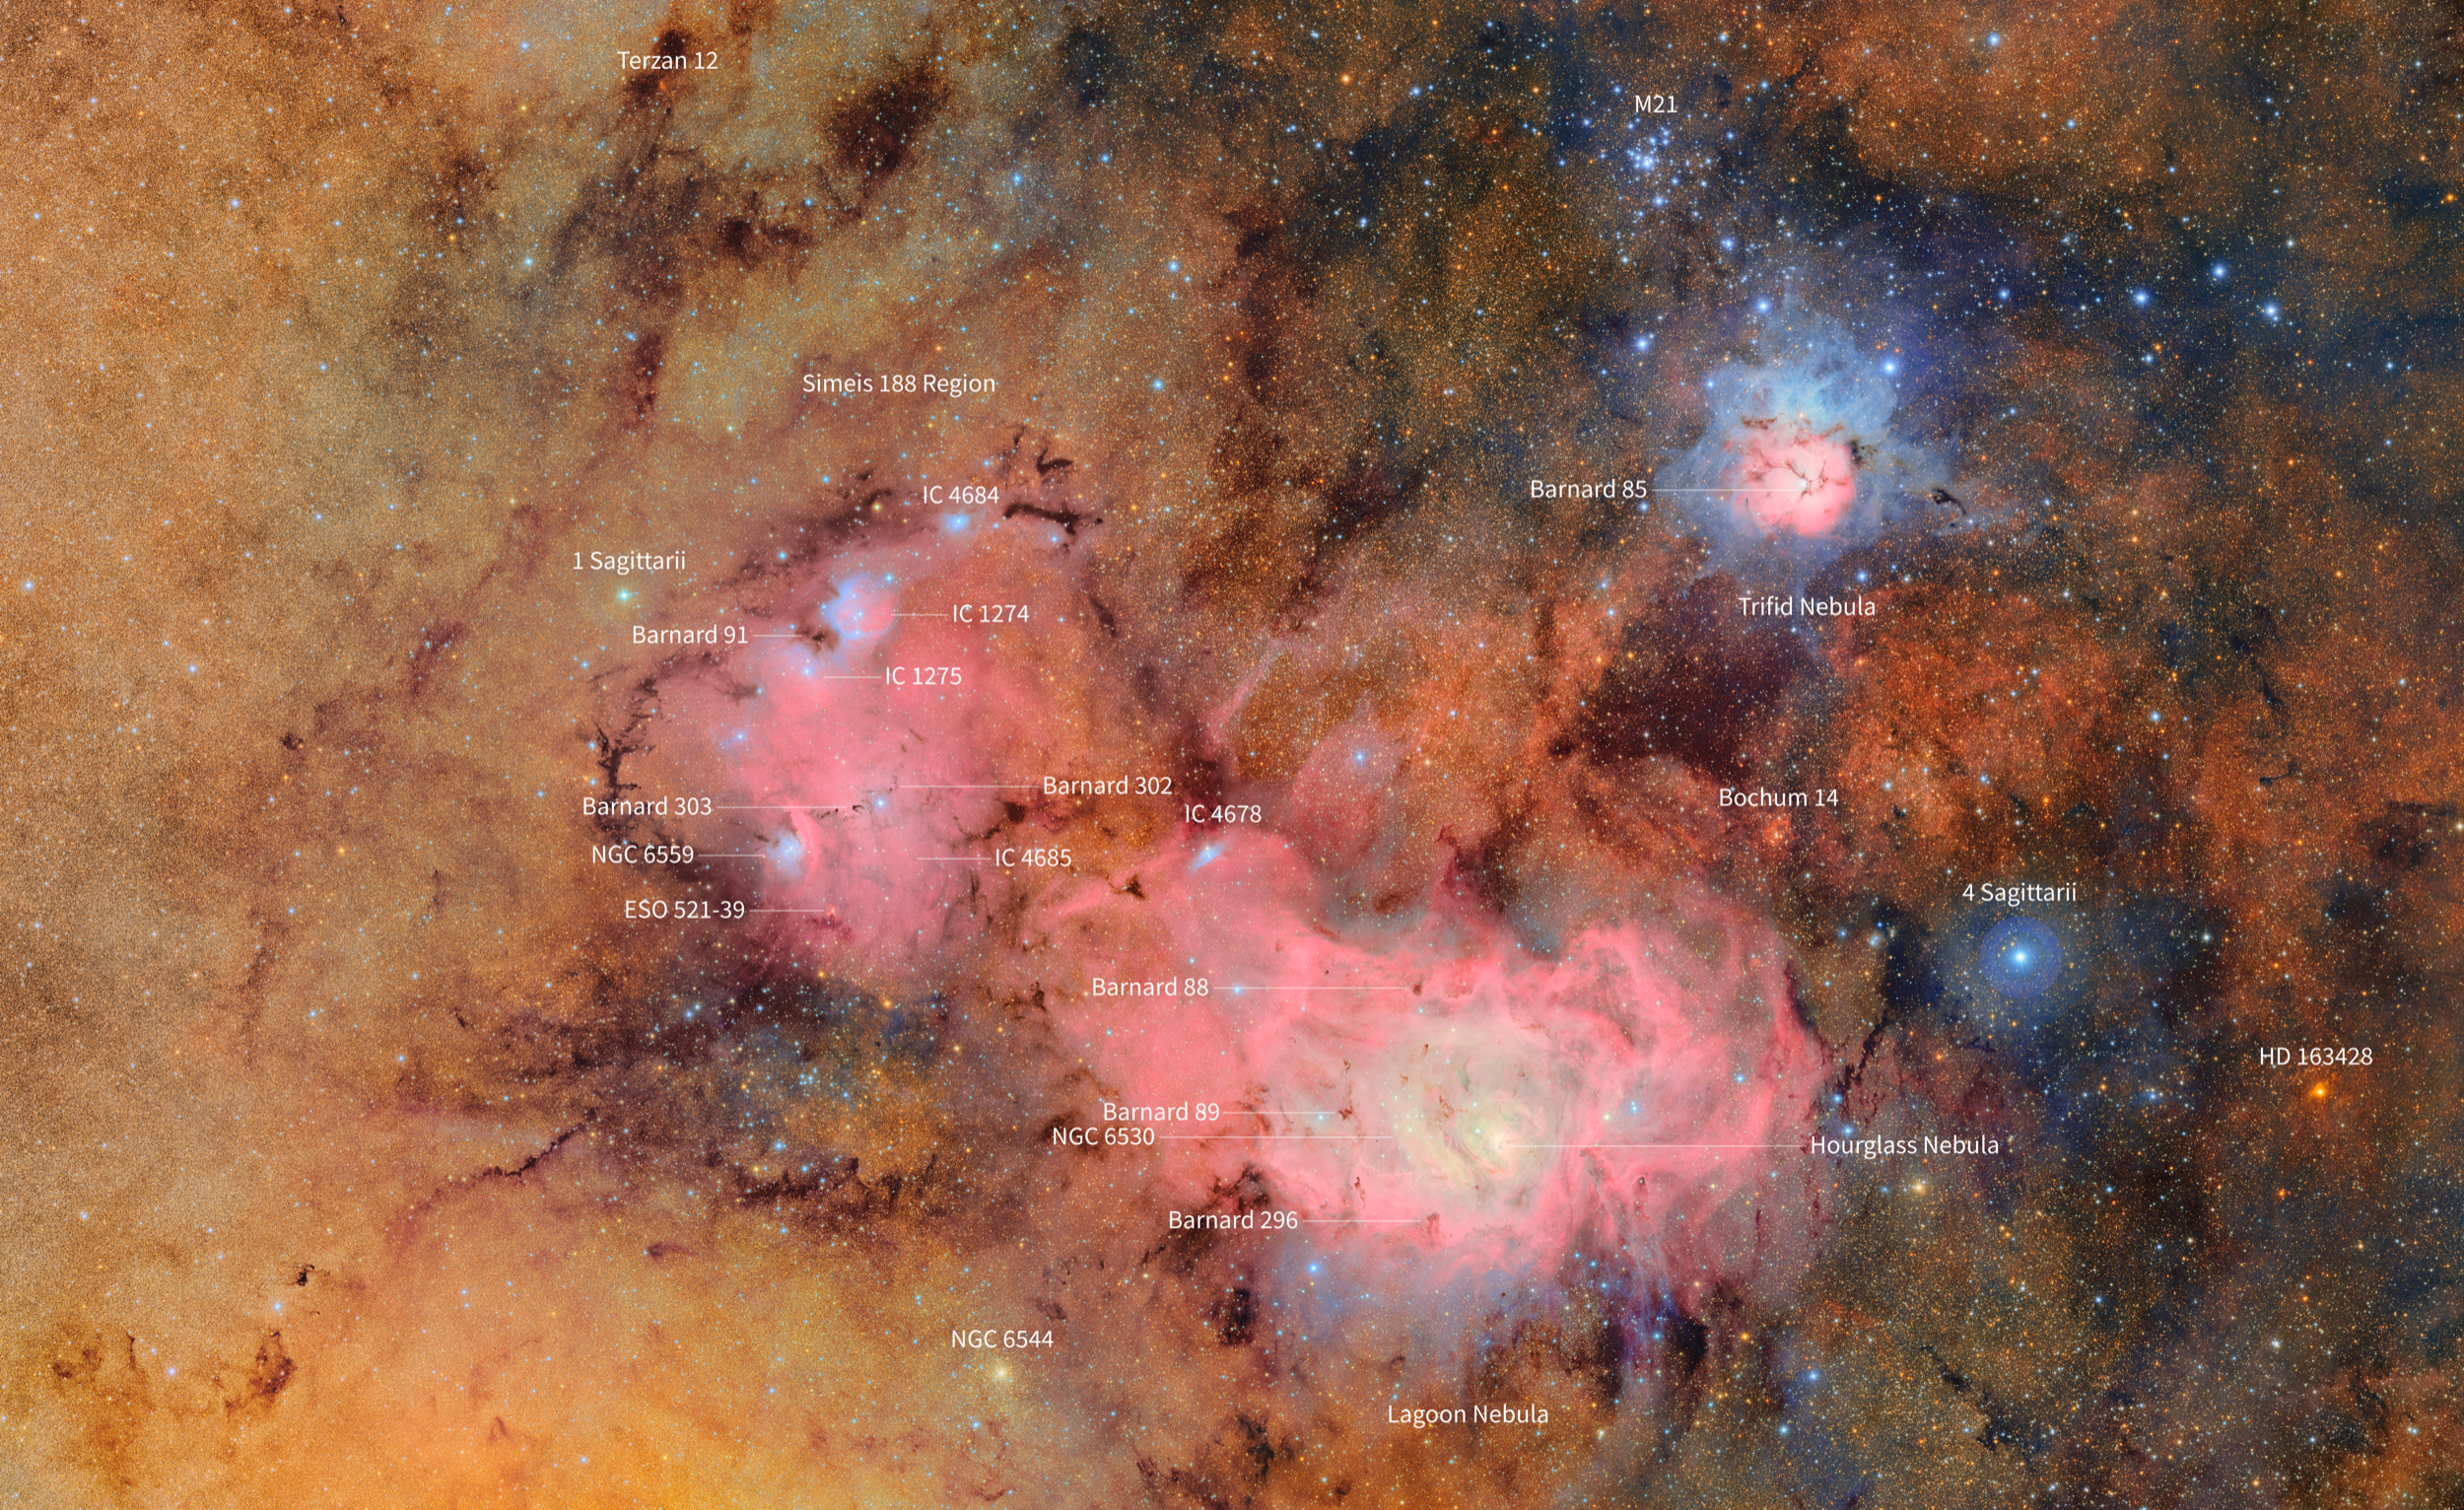
\includegraphics[width=0.9\columnwidth,clip]{Im7-10k-print}
\caption{Rubin First Look image of the Trifid (M20) and Lagoon (M8) Nebulae, combining 678 exposures taken over 7.2~hours into a $\sim$5-gigapixel mosaic.
Image credit: NSF--DOE Vera C.\ Rubin Observatory.}
\label{fig:trifid}
\end{figure}
%
\begin{figure}[htb]
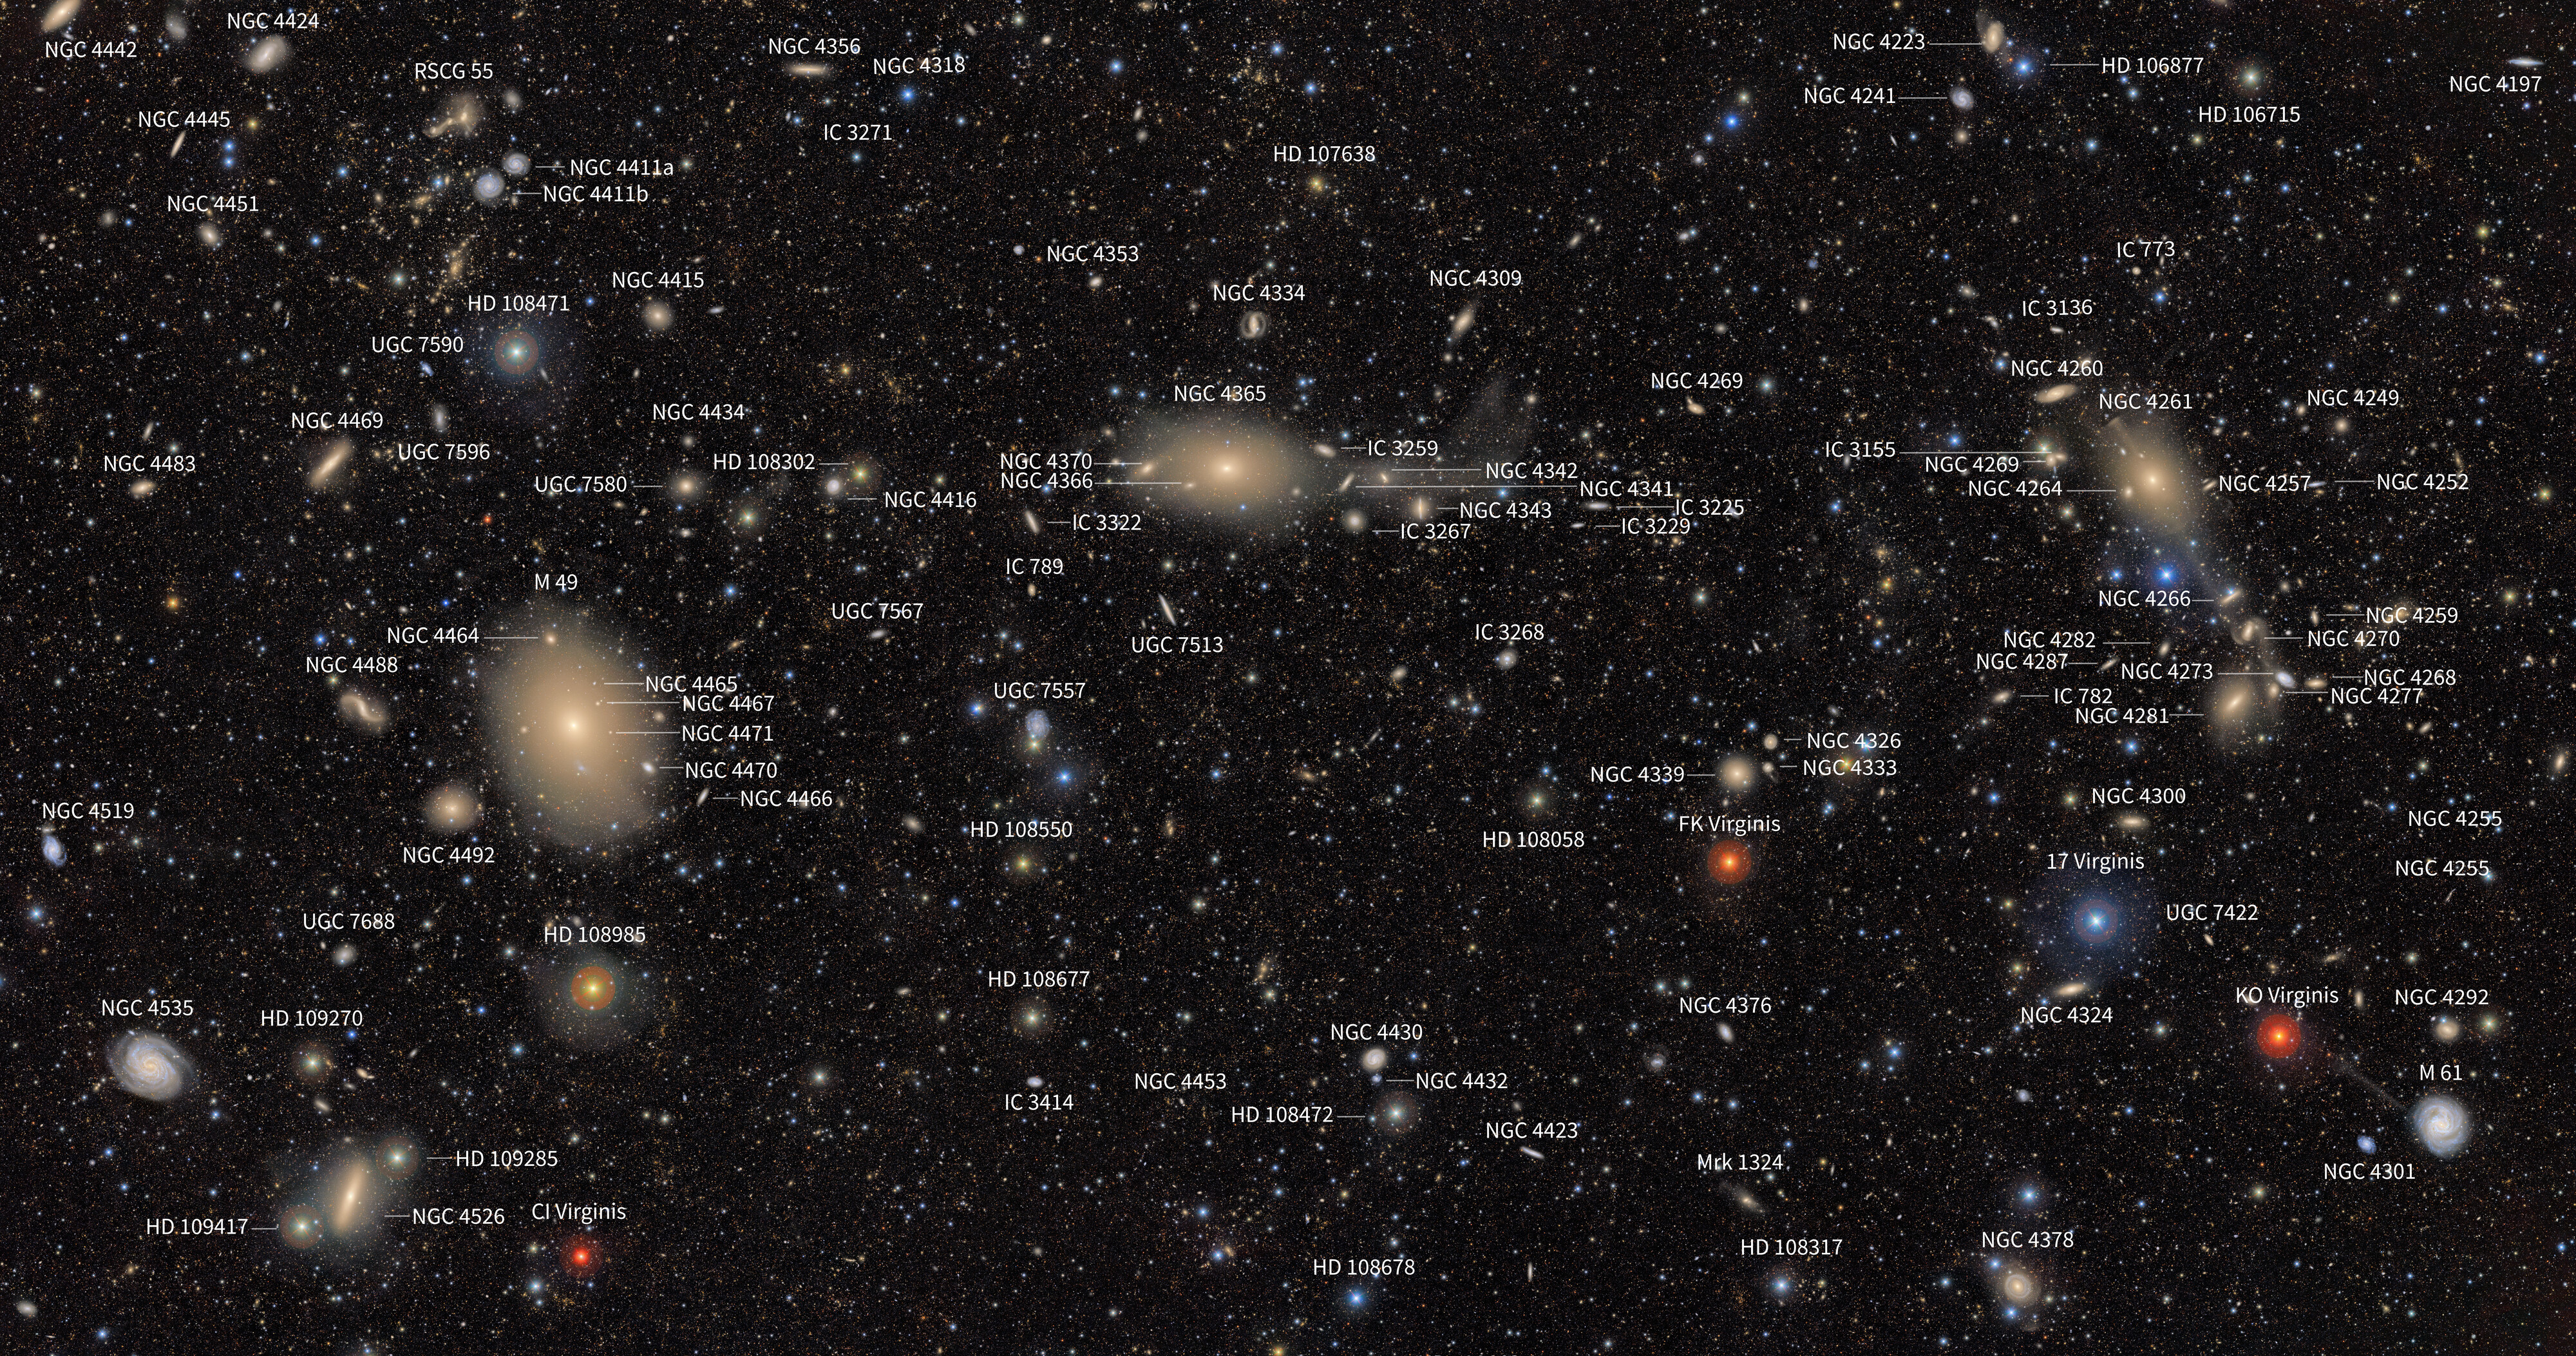
\includegraphics[width=\columnwidth,clip]{noirlab2521f}
\caption{The ``Cosmic Treasure Chest'': Rubin's First Look image of the southern Virgo Cluster around M49, combining 1\,185 images taken over 10.5~hours on seven nights and covering $\sim$25~deg$^2$.
Known objects are annotated.
Image credit: NSF--DOE Vera C.\ Rubin Observatory.}
\label{fig:treasure}
\end{figure}

The same commissioning data are already producing discoveries.
The First Look observations alone yielded 1\,514 new asteroids, and a further $\sim$11\,000, including $\sim$380 trans-Neptunian objects, were found in the commissioning surveys of mid-2025.
Rubin also observed its first interstellar object before the survey began: LSSTCam images from the Science Validation survey contain precovery detections of 3I/ATLAS (C/2025~N1)~\cite{2026ApJ..1001L..35C}, only the third interstellar object known, taken ten days before ATLAS discovered it on 1~July~2025 (Figure~\ref{fig:3IATLAS}).
With the moving-object pipelines not yet active, the detections were recovered retrospectively once the orbit was known, illustrating a general strength of wide-field surveys: repeated imaging records rare objects before their nature is recognised.
%
\begin{figure}[t]
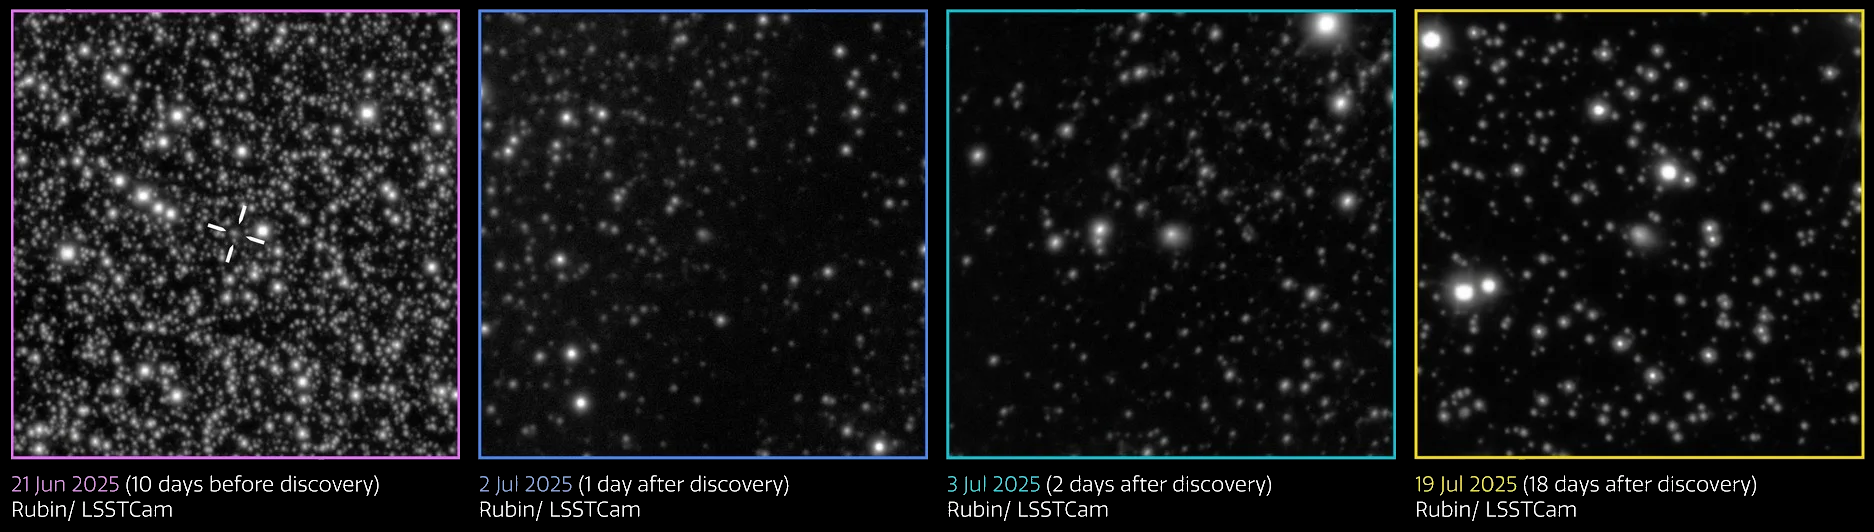
\includegraphics[width=\columnwidth,clip]{3I_ATLAS_rubin_panels}
\caption{LSSTCam images of 3I/ATLAS on 21~June 2025 (10 days before discovery, object marked), and 2, 3 and 19~July 2025 (1, 2 and 18 days after discovery).
The 21~June image is a precovery detection~\cite{2026ApJ..1001L..35C}.
Image credit: NSF--DOE Vera C.\ Rubin Observatory.}
\label{fig:3IATLAS}
\end{figure}

Before the first LSST Data Release, commissioning data reach the community through Data Previews~\cite{RTN-011}, delivered in formats representative of future releases.
Data Preview 1 (DP1)~\cite{2026AJ....171..360V} released 3.5~TB of LSSTComCam data, the first real Rubin data, and Data Preview 2 (DP2)~\cite{ RTN-115}, released on 27~July~2026 and processed entirely at the USDF, covers LSSTCam observations from April~2025 to January~2026, including the First Look fields and the 3I/ATLAS precovery images\footnote{\url{https://dp2.lsst.io}}.

% ============================================================
\section{The Rubin Data Management System}
\label{sec:ecosystem}
% ============================================================

Rubin's Data Management System (DMS), shown in figure~\ref{fig:photons_to_science}, is designed to operate as an automated, end-to-end system with minimal human intervention.
Each 30~s exposure is read out in 2~s as 205 sensor files (189 science, 8 wavefront and 8 guider), totalling $\sim$4~GB compressed ($\sim$8.2~GB uncompressed).
The survey produces $\sim$10~TB of raw data per night, with processed products far larger; the final catalog alone is projected at $\sim$15~PB.
Data are processed in two complementary streams.
\textit{Prompt Processing}~\cite{2026arXiv260319541F}, run nightly at the US Data Facility (USDF) only, is designed for speed, delivering data quickly enough to enable follow-up of transient and moving objects: each exposure is differenced against a template, and up to 10~million alerts per night distributed to seven community brokers\footnote{\url{https://rubinobservatory.org/for-scientists/data-products/alerts-and-brokers}} within 120~s, followed by catalogs within 24~h~\cite{DMTN-293} and images within 80~h.
\textit{Data Release Processing} (DRP) is optimised for quality, for science that is not time-critical: approximately once a year, the full cumulative dataset is reprocessed with the latest pipelines, producing Data Releases that are successively deeper and more precise.
%
\begin{figure}[t]
\centering
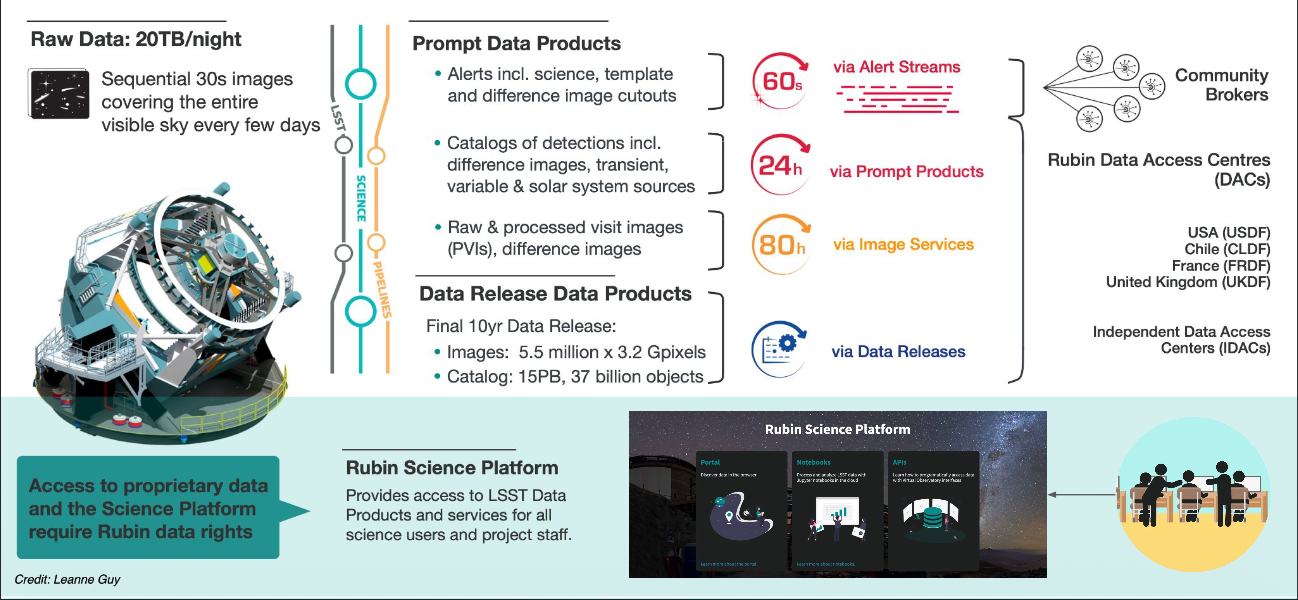
\includegraphics[width=\columnwidth,clip]{photons_to_science}
\caption{Overview of the Rubin Data Management System.
Prompt Data Products prioritise speed; Data Release Data Products prioritise quality.}
\label{fig:photons_to_science}
\end{figure}

Rubin's distributed computing layer started from the HEP tool stack (Rucio and FTS for data movement, CernVM-FS for software distribution, HTCondor for batch processing), because its data challenge resemble those of an LHC experiment (\S\ref{sec:intro}) and its data facilities already run these tools.
The central engineering challenge is a mismatch of abstraction: the Butler~\cite{2022SPIE12189E..11J}, Rubin's data middleware, manages scientific \textit{datasets} identified by instrument, sky region and observation metadata, whereas these tools operate on files identified solely by pathname.

% ============================================================
\subsection{The Distributed Data Facility Network}
\label{sec:facilities}
% ============================================================
%
Dedicated long-haul links carry each exposure from the summit to the USDF at SLAC within seconds of readout, with a three-day summit buffer protecting against network outages (Figure~\ref{fig:network}).
Annual DRP is divided across the three facilities~\cite{2024EPJWC.29501042H,2025EPJWC.33701234H}: the USDF (35\%), which hosts the archive and is the only site running Prompt Processing; the FrDF (40\%), which holds a full copy of the raw data; and the UKDF (25\%), which holds only the raw data for its assigned sky region plus the adjacent patches needed at boundaries.
CC-IN2P3 and the UK facility are long-standing WLCG sites, so the infrastructure, expertise and staff experience needed to run HEP tools are already in place.

Inter-site connectivity is provided by ESnet, G\'{E}ANT, JANET and RENATER, with transatlantic round-trip times of up to $\sim$165~ms.
Data movement falls into three domains~\cite{2025EPJWC.33701129H}: latency-critical transfer from the summit to the USDF ($\sim$4~TB per night compressed); volume-critical replication between facilities, with $\sim$2~PB of raw data flowing each year from the USDF to Europe and $\sim$20~PB of processed products flowing back; and scale-critical distribution of multi-PB releases to Independent Data Access Centers (IDACs) (\cite{RTN-003, RTN-104}) that host published data products.
%
\begin{figure}[h]
\centering
\includegraphics[width=\columnwidth,clip]{rubin_network_dataflow}
\caption{The Rubin network and data flow: raw images travel from the summit to the USDF for Prompt Processing and archiving, are replicated to the FrDF (40\%) and UKDF (25\%) for Data Release Processing, processed products return to the archive, and releases are distributed to IDACs worldwide.}
\label{fig:network}
\end{figure}

The sky is partitioned into tracts of $\sim$1.6$^\circ$ on a side, each divided into a $7\times7$ grid of $\sim$13.7~arcmin patches with overlaps between neighbours.
Each facility receives its assigned tracts plus a buffer of adjacent patches for objects that straddle a boundary, such as bright stars, extended galaxies and moving asteroids; small overlap regions are processed at all three facilities and compared as numerical consistency checks before each release.
All processing is orchestrated centrally from the USDF, including jobs that execute at remote facilities.

The USDF, Rubin's allocation within SLAC's Shared Scientific Data Facility (S3DF), has 145 batch nodes ($\sim$17,400 cores, $\sim$21,600 Milano-equivalent) and $\sim$30~PB of installed disk, representative of the scale at each facility; beyond the batch and storage tier, the USDF hosts a 92-node Qserv cluster for catalog queries and a 12-node Cassandra cluster for the Alert Production Database (APDB).
DP2 consumed $\sim$970 node-days ($\sim$2.8~million core-hours) to process $\sim$30,000 visits; DR1 is estimated at $\sim$35~million core-hours ($\sim$12,000 node-days), growing linearly with each subsequent release.

% ============================================================
\subsection{Summit to US Data Facility}
\label{sec:summit-usdf}
% ============================================================

The summit is connected to SLAC by a 100/40~Gbps primary/backup long-haul link with hardware-accelerated IPsec encryption.
Each exposure must reach the USDF within $\sim$7~s so that Prompt Processing can finish within its 120~s budget; a new exposure follows every $\sim$35--40~s.
Transfer is handled by \texttt{s3nd} (Deliverator), a small custom Go daemon that writes all 205 sensor files in parallel to an S3-compatible object store at the USDF, keeping a pool of persistent connections open to avoid the TLS handshake and TCP slow-start cost on every file over a high-latency international link.
A listener at the USDF watches the bucket, triggers Butler ingestion, and launches Prompt Processing as each exposure arrives.
In early operations, 80\% of exposures arrive within 7~s; the tail stems from several causes, including network failover, camera retransmission, and queueing at the shared USDF object store.
Telemetry from the Engineering Facility Database (EFD) is transferred as messages via Sasquatch~\cite{2024SPIE13101E..1MF}, a Kafka-based system, and certified calibration products are returned from the archive to the summit via rsync at $\mathcal{O}(100)$~GB~day$^{-1}$.

% ============================================================
\subsection{Science Pipelines, Middleware, and Workflow Orchestration}
\label{sec:pipelines}
% ============================================================
%
The LSST Science Pipelines~\cite{PSTN-019} implement the scientific algorithms, from instrument signature removal through calibration, coaddition and difference imaging to catalog production.
All input and output passes through the Butler~\cite{2022SPIE12189E..11J}, which hides file locations and formats from algorithm developers: tasks access data by scientific identifier (instrument, visit, detector, band, sky region), never by file path, and each repository combines
% TODO: Comment from Tim needs checking -- "I thought the European sites were all using WebDAV and not using POSIX."
a relational registry with a datastore on POSIX, WebDAV or S3-compatible storage.

The Batch Processing System (BPS) (\cite{2025ASPC..538..325G}) queries the Butler registry and builds a Quantum Graph, a directed acyclic graph in which each node is one \texttt{PipelineTask} applied to one unit of data; for a full release campaign it contains millions of nodes.
BPS translates the graph into batch jobs through pluggable backends.
The primary backend is HTCondor: BPS submits directly from the USDF to the European facilities, whose batch resources are exposed through ARC-CE over SLURM (FrDF) and HTCondor (UKDF), providing cross-site orchestration through the same interface as at the USDF, without a dedicated pilot system.
Rubin used PanDA~\cite{2024EPJWC.29504026K} through commissioning, DP1 and DP2, which validated centralised cross-site submission and the separation of workflow description from execution environment.
Rubin now favors BPS with HTCondor because the Quantum Graph already encodes all data dependencies and provenance, so a lightweight submission layer built around Butler's data model suffices, rather than a general-purpose workload management system.
PanDA remains a validated alternative backend for workflows that require richer workload management.

The Science Pipelines, with their configuration and static calibration data, are built once and distributed via CernVM-FS (Stratum-0 at FrDF, Stratum-1 replicas elsewhere) to all data facilities, IDACs and Rubin Science Platform deployments, so that identical code runs everywhere, a prerequisite for the cross-facility consistency checks.

\subsection{Multi-site Data Movement: Rucio, FTS, and HermesK}
\label{sec:rucio}
% ============================================================

Rubin operates a dedicated Rucio and FTS instance for all inter-facility data movement.
Raw images are replicated daily from the USDF, with a 3-day embargo delay (see~\cite{DMTN-199}), to the European facilities; each day's $\sim$1\,000 exposures are bundled into a single $\sim$4~GB zip archive of per-detector FITS files.
Bundling simplifies transfer and archiving for Rucio and FTS~\cite{2025EPJWC.33701129H} but adds complexity to the Butler and the data access services, which must index and retrieve individual files within each archive.

Each facility exposes two Rucio Storage Elements (RSEs), one for inputs and one for processing outputs, which allows transfers to be prioritised and protects the irreplaceable raw data.
The harder direction is returning processed products to the USDF: processing expands the data volume by up to a factor of ten, producing from each raw image many new, smaller data products (KB to 100~MB).
Unlike raw ingest, processed outputs are not re-bundled, so each zipped raw expands into 189 separate output files, which Rucio and FTS handle poorly at this scale (\S\ref{sec:challenges}).

Butler and Rucio are connected by two components (Figure~\ref{fig:butler_rucio}).
At the sending side, \texttt{rucio\_register}, run by final pipeline jobs, registers output files from the Butler into Rucio datasets (collections of files), attaching $\sim$500~bytes of science metadata per file directly to the Rucio record so that no separate sidecar file is needed; pre-configured subscription rules then trigger replication.
Only final data products are registered; intermediates, which can outnumber them tenfold, stay local.
One exception is the DR1 global calibration step, which requires a mid-campaign round trip: per-visit star catalogs and visit summaries travel from each facility to the USDF, and the resulting calibration products are returned to all sites before processing can continue.
Developers also occasionally need intermediate products at the USDF for debugging.
This round trip is the strongest argument for event-driven ingest over polling (\S\ref{sec:challenges}).

At the receiving side, a file delivered by FTS lands in storage but is invisible to the local Butler, so no pipeline can use it.
HermesK~\cite{2025EPJWC.33701129H}, a modified Rucio Hermes daemon, closes this gap.
Like the rest of Rucio, it runs centrally at the USDF, and all Kafka traffic originates there.
HermesK watches the Rucio database for Rubin transfer-completion events, attaches the Rubin metadata, and publishes each event to a Kafka topic named after the destination RSE recorded in the event.
Each facility subscribes only to its own topic, so it receives only messages it can act on; each event carries the data ID, filename, UUID and science metadata, and \texttt{ctrl\_ingestd} ingests each arriving file into the local Butler, making it available for processing without polling.
This holds provided the corresponding Butler dimension records already exist at the destination; if they are absent, ingestion fails.
Calibration collections and chained collection definitions are not propagated by events and are currently rebuilt by hand.
Kafka was chosen over ActiveMQ, which Hermes already supports, because Kafka's MirrorMaker provides cross-site message replication out of the box and Rubin already had extensive Kafka expertise, including from its EFD telemetry system.

% Update status before submission
HermesK is an interim solution.
A pull request under review adds generic Kafka messaging to the upstream Hermes daemon, analogous to its existing ActiveMQ support, while the Rubin-specific event filtering has moved into a separate, completed daemon, \texttt{ctrl\_filterd}.
Once the pull request is accepted, Rubin will retire HermesK and run the standard Hermes daemon with Kafka, removing the need to patch each Rucio release.
%
\begin{figure}[t]
\centering
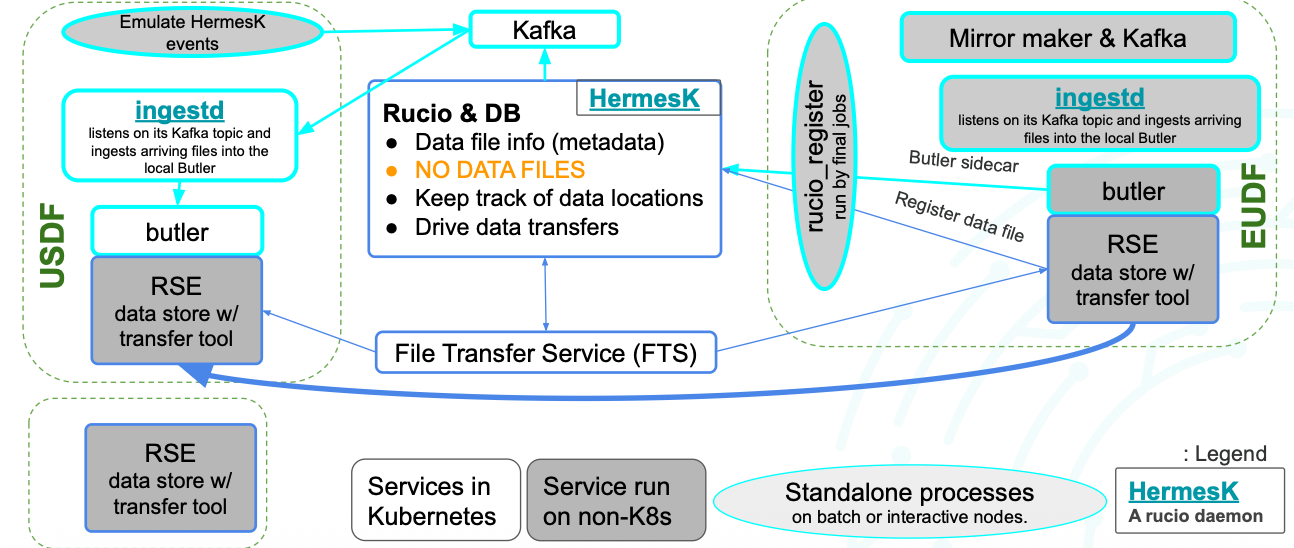
\includegraphics[width=\columnwidth,clip]{data_registration_compact}
\caption{Data flow from pipeline output to cross-site ingestion: \texttt{rucio\_register} registers final products with Rubin metadata in Rucio, FTS transfers them, HermesK publishes completion events to per-RSE Kafka topics, and \texttt{ctrl\_ingestd} ingests each file into the receiving Butler.}
\label{fig:butler_rucio}
\end{figure}
%
% ============================================================
\subsection{Data Distribution to the Science Community}
\label{sec:distribution}
% ============================================================

Each annual release will be distributed from the USDF archive to 15--20 IDACs~\cite{2024EPJWC.29507017M} across the Americas, Europe and the Asia-Pacific region.
An IDAC needs only a storage endpoint compatible with Rucio and FTS; orchestration is managed centrally at the USDF, which prevents simultaneous downloads from congesting the archive, and transfers can also run between IDACs.
DP1 (3.5~TB) was distributed to 9 IDACs in this way, with Globus used for NERSC~\cite{2026AJ....171..360V,RTN-086}, and the same infrastructure is being scaled to DP2 ($\mathcal{O}(100)$~TB) and to petabyte-scale Data Releases.
Scientists access the data through the Rubin Science Platform~\cite{2024SPIE13101E..2BO}, where, as in HEP, they bring their analysis to the data rather than downloading it.

% ============================================================
\section{Open challenges and cross-disciplinary lessons}
\label{sec:challenges}
% ============================================================

DR1 will be the first full LSST release: an end-to-end multi-site campaign over $\sim$5~PB of raw data from the first year of the survey, with automated data movement in both directions across all three facilities.
The components described in \S\ref{sec:ecosystem} have been exercised individually during commissioning and the DP2 pilot campaigns at FrDF; no end-to-end campaign has yet run across all three sites at DR1 scale, and doing so reliably and repeatedly is the remaining challenge.
Deploying them has exposed friction points that are instructive for any experiment crossing the HEP--astronomy boundary.

The most important enabling factor was institutional overlap.
All three Rubin data facilities already operated these tools for the LHC (\S\ref{sec:facilities}), so their systems, network and storage teams brought direct operational experience with Rucio, FTS and HTCondor, and Rubin staff with backgrounds in ATLAS, LHCb and CERN grid computing turned this proximity into practical deployment.

The principal challenge is the file-count regime.
In HEP, events are aggregated into multi-GB files, so per-file overheads are small relative to the data volume.
In Rubin, the natural unit is the detector image: each visit comprises 189 science detectors processed independently, and every pipeline quantum writes its outputs (images, catalogs, metadata, logs and provenance) as separate Butler-tracked files.
File counts therefore reach billions per Data Release, many in the KB to few-MB range, a regime in which the file-oriented HEP tools struggle.
Current mitigations are bundling per-quantum outputs into zip archives and not persisting intermediate products, and returning processed outputs from the European facilities to the USDF archive remains on the critical path for DR1.
S3 object storage at the USDF avoids POSIX inode limits, but bridging it to POSIX storage at the European facilities remains an active engineering problem; more broadly, object storage combined with a science-metadata layer such as the Butler is a concrete alternative for any workload, in astronomy or HEP, that produces many small outputs.

The second challenge is keeping the Butler's dataset model consistent with the file-oriented tools across three independent sites, and it is directly connected to the small-file problem: both difficulties trace back to having two independent systems that each record where a file resides.
Each site's Butler registry knows only about locally present files.
HermesK and \texttt{ctrl\_ingestd} (\S\ref{sec:rucio}) automate file arrival for datasets whose dimension records already exist at the destination; ensuring that calibration updates are propagated and acknowledged at every site before a campaign, which cannot be done by polling at Data Release scale, is an active area of development.
Verifying end-to-end completeness also remains open: Rucio tracks whether a file has been transferred, but not whether it has been successfully ingested into the local Butler, leaving no unified view of what is actually available for processing at each site.
The large file counts compound the problem at campaign end: retiring intermediate products requires purging records from both Rucio and the Butler registry, an operation that is slow at this scale.
Extending Butler to carry multi-site location information natively is one approach under active consideration.
Keeping dimension records current across sites adds a further layer of complexity: when a header error is identified after ingest, the correction must be applied to Butler's dimension records at every facility, a synchronisation problem with no equivalent in the single-registry HEP model.

% ============================================================
\section{Conclusions}
\label{sec:conclusions}
% ============================================================

Rubin Observatory is operational and delivering science.
Since first on-sky images in April 2025, the Data Management System has transferred more than 90\,000 science-quality images from the summit in Chile to data facilities on three continents, issued millions of alerts per night, and produced two Data Previews.
Even before the survey began, these data led to the discovery of more than 11\,000 new asteroids, including $\sim$380 trans-Neptunian objects, and captured the third known interstellar object, 3I/ATLAS, ten days before it was discovered.

These results were achieved in collaboration with the HEP community and with HEP tools: Rucio and FTS for data movement, CernVM-FS for software distribution, and HTCondor, via BPS, for processing, building on experience gained with PanDA.
Rubin's principal contribution back is Kafka messaging for the Rucio Hermes daemon, developed for HermesK, which makes Rucio's file-level transfers visible to the Butler without polling and is available to any experiment with similar requirements.
The remaining challenges, chiefly the small-file regime and cross-site Butler consistency, are well understood and are being addressed for DR1; beyond DR1 the load grows every year, as each release reprocesses the entire cumulative dataset.
Rubin's experience so far suggests that adopting and extending HEP infrastructure is a sound model for the next generation of data-intensive astronomical facilities.


\section*{Acknowledgements}

This material is based upon work supported in part by the National Science Foundation through Cooperative Agreements AST-1258333 and AST-2241526 and Cooperative Support Agreements AST-1202910 and AST-2211468 managed by the Association of Universities for Research in Astronomy (AURA), and the Department of Energy under Contract No.\ DE-AC02-76SF00515 with the SLAC National Accelerator Laboratory managed by Stanford University.
Additional Rubin Observatory funding comes from private donations, grants to universities, and in-kind support from LSST-DA Institutional Members.
This work has been supported by the French National Institute of Nuclear and Particle Physics (IN2P3) through dedicated funding provided by the National Center for Scientific Research (CNRS).

%% Appendix material should be preceded with a single \appendix command.
%% There should be a \section command for each appendix.
%% \appendix

% Include all the relevant bib files.
% https://lsst-texmf.lsst.io/lsstdoc.html#bibliographies
\bibliography{local,lsst,lsst-dm,refs_ads,refs,books}

\end{document}

